%!TEX root = ../thesis.tex
%*******************************************************************************
%*********************************** Results *********
%*******************************************************************************


\chapter{Results}

\ifpdf
    \graphicspath{{chapter-results/Figs/Raster/}{chapter-results/Figs/PDF/}{chapter-results/Figs/}}
\else
    \graphicspath{{chapter-results/Figs/Vector/}{chapter-results/Figs/}}
\fi



\section{Background-only}\label{sec:results_background_only}



 \begin{figure}
	\centering
	\begin{subfigure}[b]{0.5\linewidth}
		\centering\includegraphics[width=0.85\textwidth]{OneLeptonbb_CR_TRLMEM_mct2_yellow}
	\end{subfigure}\hfill
	\begin{subfigure}[b]{0.5\linewidth}
		\centering\includegraphics[width=0.85\textwidth]{OneLeptonbb_CR_TRMMEM_mct2_yellow}
	\end{subfigure}\hfill
	\begin{subfigure}[b]{0.5\linewidth}
		\centering\includegraphics[width=0.85\textwidth]{OneLeptonbb_CR_TRHMEM_mct2_yellow}
	\end{subfigure}\hfill
	\begin{subfigure}[b]{0.5\linewidth}
		\centering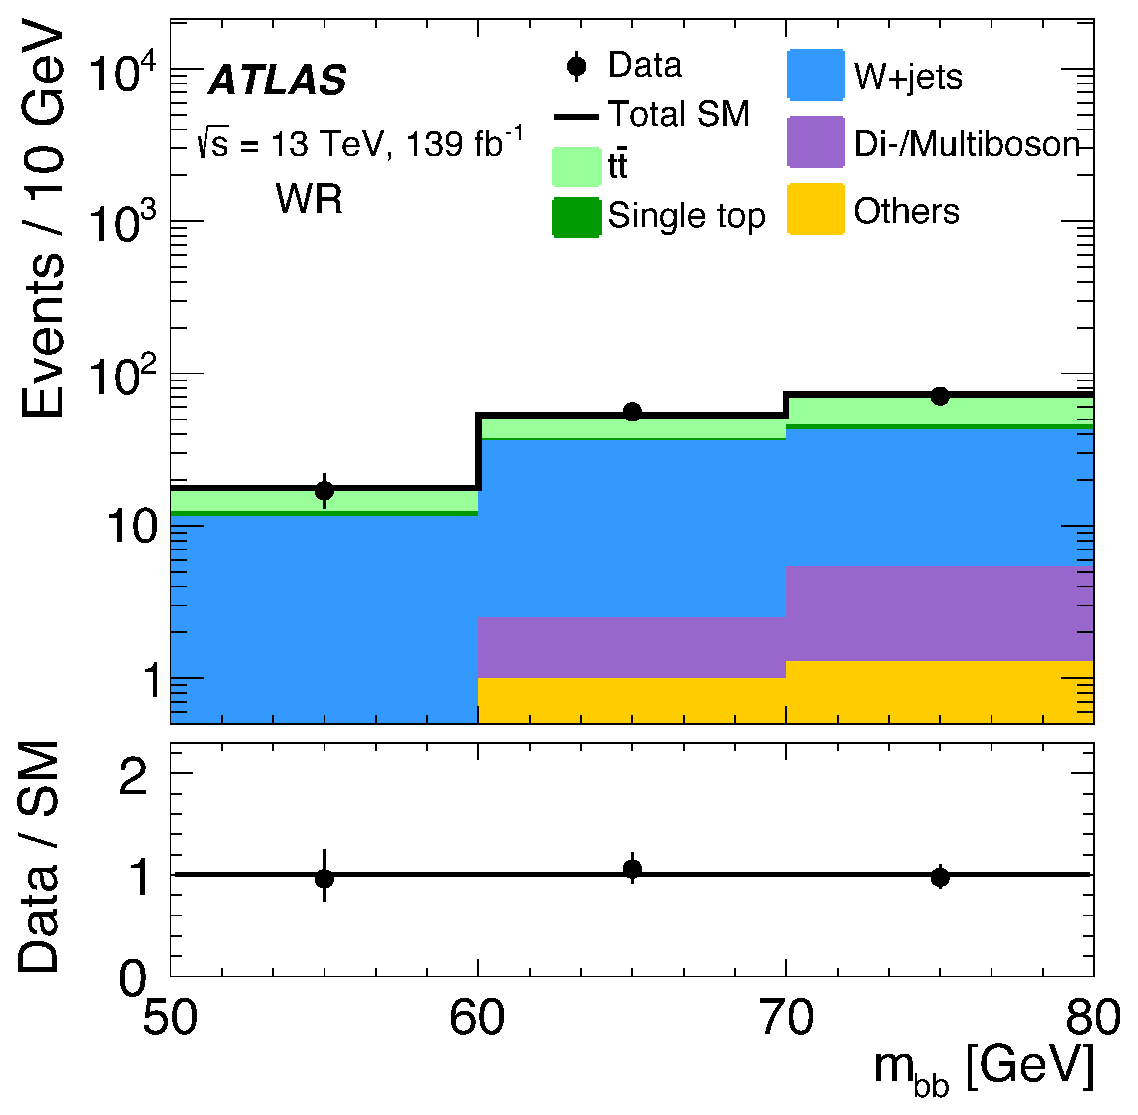
\includegraphics[width=0.85\textwidth]{OneLeptonbb_CR_WREM_mbb_yellow}
	\end{subfigure}\hfill
	\begin{subfigure}[b]{0.5\linewidth}
		\centering\includegraphics[width=0.85\textwidth]{OneLeptonbb_CR_STCREM_mbb_yellow}
	\end{subfigure}\hfill

	\caption{Exemplary distribution shown in each control region after the background-only fit. The shaded region includes all systematic uncertainties (including correlations) as well as \gls{mc} statistical uncertainty. The $\ttbar$, single top and $\wjets$ are normalised simultaneously in all \glspl{cr}. A good agreement between \gls{mc} expectation and data is observed in all \glspl{cr}.}
	\label{fig:CR_distributions_postfit}
\end{figure}


\section{Validation regions}



 \begin{figure}
	\centering
	\begin{subfigure}[b]{0.5\linewidth}
		\centering\includegraphics[width=0.85\textwidth]{OneLeptonbb_VR_UnderFlowBin_VRtt1offnomct2EM_mct2_yellow}
	\end{subfigure}\hfill
	\begin{subfigure}[b]{0.5\linewidth}
		\centering\includegraphics[width=0.85\textwidth]{OneLeptonbb_VR_UnderFlowBin_VRtt1onnomct2EM_mct2_yellow}
	\end{subfigure}\hfill
	\begin{subfigure}[b]{0.5\linewidth}
		\centering\includegraphics[width=0.85\textwidth]{OneLeptonbb_VR_UnderFlowBin_VRtt2offnomct2EM_mct2_yellow}
	\end{subfigure}\hfill
	\begin{subfigure}[b]{0.5\linewidth}
		\centering\includegraphics[width=0.85\textwidth]{OneLeptonbb_VR_UnderFlowBin_VRtt2onnomct2EM_mct2_yellow}
	\end{subfigure}\hfill
	\begin{subfigure}[b]{0.5\linewidth}
		\centering\includegraphics[width=0.85\textwidth]{OneLeptonbb_VR_UnderFlowBin_VRtt3offnomct2EM_mct2_yellow}
	\end{subfigure}\hfill
	\begin{subfigure}[b]{0.5\linewidth}
		\centering\includegraphics[width=0.85\textwidth]{OneLeptonbb_VR_UnderFlowBin_VRtt3onnomct2EM_mct2_yellow}
	\end{subfigure}\hfill

	\caption{Exemplary distributions shown in each validation region after the background-only fit with subsequent extrapolation to the \glspl{vr}. All selection cuts except for the requirement on $\mct$ (indicated using the red arrow) are applied. The shaded region includes all systematic uncertainties as well as \gls{mc} statistical uncertainty.}
	\label{fig:VR_distributions_postfit}
\end{figure}

\section{Signal regions}



 \begin{figure}
	\centering
	\begin{subfigure}[b]{0.5\linewidth}
		\centering\includegraphics[width=0.85\textwidth]{OneLepton_Wh_SRLMEM_mct2_yellow}
	\end{subfigure}\hfill
	\begin{subfigure}[b]{0.5\linewidth}
		\centering\includegraphics[width=0.85\textwidth]{OneLepton_Wh_SRMMEM_mct2_yellow}
	\end{subfigure}\hfill
	\begin{subfigure}[b]{0.5\linewidth}
		\centering\includegraphics[width=0.85\textwidth]{OneLepton_Wh_SRHMEM_mct2_yellow}
	\end{subfigure}\hfill

	\caption{Exemplary distribution shown in each exclusion signal region after the background-only fit. The shaded region includes all systematic uncertainties (including correlations) as well as \gls{mc} statistical uncertainty.}
	\label{fig:SR_distributions_postfit}
\end{figure}

\section{Interpretation}

